\documentclass[12pt, openany, twoside]{report}      % paper size is in preamble.sty

%\usepackage[utf8x]{inputenc}
%\renewcommand*\sfdefault{ugq}
\usepackage[T1]{fontenc}
\usepackage{lmodern}
\usepackage{graphicx}
\usepackage{booktabs}
\usepackage{amsfonts}
\usepackage{multicol}
\usepackage{microtype}
%\usepackage[a4paper]{geometry}
\usepackage[top=1in, bottom=1.25in, left=0.5in, right=0.5in]{geometry}

\def\TITLE{NORDAN 26}
\def\SUBTITLE{Nordic Complex Analysis Meeting}
\def\LOCATION{Hella, Iceland -- May 23-25, 2025}

\begin{document}
\begin{titlepage}
    \centering
    %\vpspace{3cm}
    
\includegraphics[scale = 1.00]{figs/kaus-title} \\
    \vfill
    \vfill
    
\includegraphics[scale = 1.00]{figs/kaus-loc}\par\vspace{1cm}
    \vfill
    \vfill
    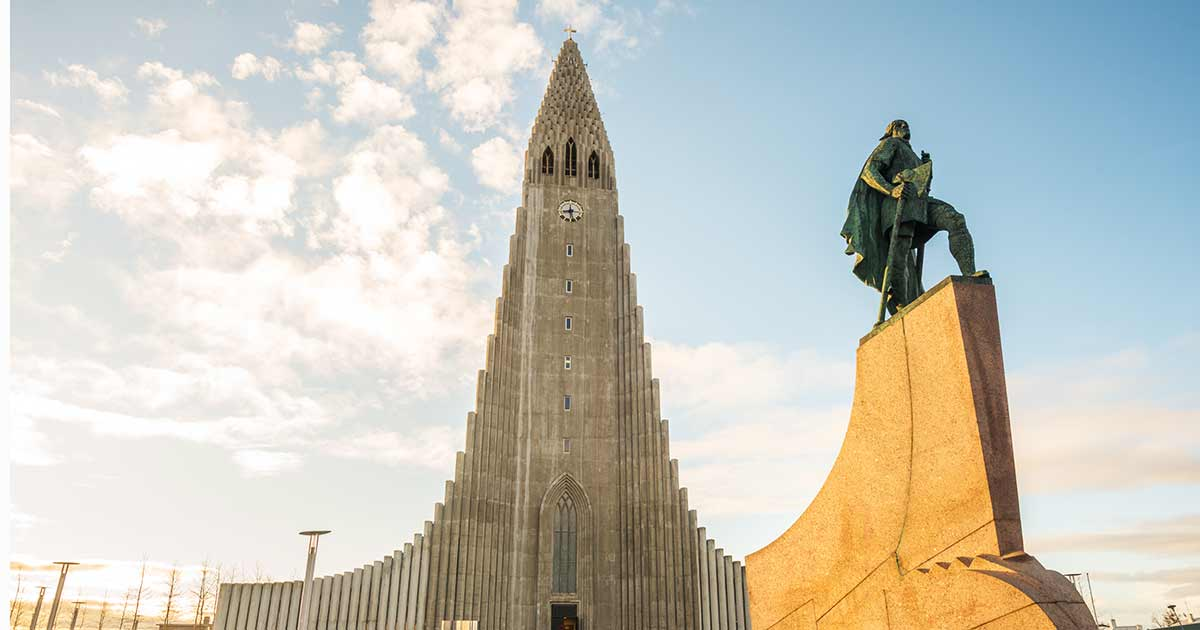
\includegraphics[width=0.8\textwidth]{figs/hallgrimskirkja}\par\vspace{1cm}
    \vfill
    \vfill
\end{titlepage}

\renewcommand{\arraystretch}{1.2}
%\usepackage[top=1in, bottom=1.25in, left=0.5in, right=0.5in]{geometry}
\newgeometry{top = 1 in}

\noindent
{\LARGE Program}

\bigskip
\bigskip
\noindent
\textbf{\large Thursday, May 22nd}
\smallskip

\noindent
\begin{tabular}{l@{ } l@{ } l l}
16:30 & - & 16:55 & \textsc{Suprokash Hazra}
\\
17:00 & - & 17:25 & \textsc{Rahim Nkunzimana}
\\
17:30 & - & 17:55 & \textsc{Benjamin Marim de Moura}
\\
18:00 &  &  & \textit{Activities}
\end{tabular}

\bigskip
\noindent
\textbf{\large Friday}
\smallskip

\noindent
\begin{tabular}{l@{ } l@{ } l l}
10:00 & - & 10:25 & \textsc{Gaofeng Huang}
\\
10:30 & - & 10:55 & \textsc{Fani Xerakia}
\\
11:00 & - & 11:25 & \textsc{Ai My Aleksandra Le}
\\
11:30 & - & 12:30 & \textit{Lunch}
\\
12:30 & - & 12:55 & \textsc{Ludvig Svensson}
\\
13:00 & - & 13:25 & \textsc{Rolf Andreasson}
\\
13:30 & - & 13:55 & \textsc{Johannes Testorf}
\\
14:00 & - & 14:30 & \textit{Break}
\\
14:30 & - & 14:55 & \textsc{Setareh Eskandari}
\\
15:00 & - & 15:25 & \textsc{Beno Učakar}
\\
15:30 & - & 15:55 & \textsc{Atte Pennanen}
\end{tabular}




\vfill
\vfill
\noindent
Organizers:
\begin{itemize}
    \setlength\itemsep{-0.3 em}
    \item Tryggvi Kalman Jónsson, Háskóli Íslands
    \item Mar Saiz Aparicio, Universitetet i Stavanger
\end{itemize}
\vfill

\cleardoublepage

\newcommand\talk[3]{%
    \vspace{7 ex}
    \noindent
    \textsc{\large #1}

    \smallskip
    \noindent
    \textbf{\textit{#2}}

    \medskip
    \noindent
    #3

}

\talk
{%
    Rahim Nkunzimana
}
{%
    Holomorphic matrices -- an argument principle
}
{%
    Suppose $f$ is a matrix of holomorphic functions in several
    variables. If $f$ is surjective outside the origin, one can define
    the Buchsbaum-Rim multiplicity of $f$, generalising the order of
    vanishing of a single variable function. We show that we get a
    representation of the Buchsbaum-Rim multiplicity as a product of
    a smooth form and a residue current. This can be seen as an
    argument principle for holomorpic matrices, and it generalises a
    result of Andersson, where row matrices were considered, as well
    as a previous result of the speaker, where direct sums of row
    matrices were considered. 
}

\talk
{%
    Ludvig Svensson
}
{%
    Critical inverse temperatures as solutions\\to discrete optimization problems
}
{%
    \looseness=-1
    Consider a system of $N$ point particles at positions
    $p_1, \dots, p_N$ on the $2$-dimensional sphere $\mathbb{S}^2$
    that interact according to the \emph{Coulomb potential}
    \[
        E = \sum_{1\leq i<j\leq N}c_{i,j}\log\|p_i - p_j\|^2,
    \]
    where $c_{i,j}$ is a symmetric matrix of real coupling constants,
    describing the strength (and sign) of interaction between
    particle $i$ and particle $j$.
    In joint work together with Rolf Andreasson, we use tools from
    Complex and Algebraic geometry to study the
    \emph{Gibbs measure} and associated
    \emph{partition function} of this system in thermal
    equilibrium at inverse temperature $\beta$. We show that the
    critical inverse temperature(s), where the partition function
    diverges, are solution(s) to a certain discrete optimization
    problem.
}

\talk
{%
    Fani Xerakia
}
{%
    Automorphisms of the Worm Domain
}
{%
    The Diederich-Fornæss worm domain, constructed as the first
    smoothly bounded pseudoconvex domain without a Stein
    neighbourhood basis, is a key counterexample in Several
    Complex Variables. In this talk, we examine its automorphism
    group in both bounded and unbounded cases and demonstrate that
    its boundary is locally spherical everywhere except at the
    exceptional locus and the caps.
}

\newpage
\talk
{%
    Gaofeng Huang
}
{%
    Large holomorphic automorphism groups
}
{%
    In this talk, we survey a few results in the study of large
    holomorphic automorphism groups. First we give an historical
    account of the so-called Andersen-Lempert theory, the core of
    which is an approximation of local biholomorphic injections by
    global holomorphic automorphisms, developed by Andersen-Lempert
    and Forstneric-Rosay in the 90s. Such an approximation is
    possible on Stein manifolds with the density property, a
    property describing the abundance of globally integrable
    holomorphic vector fields.  It thus is fundamental to identify
    Stein manifolds with this property. A criterion by Kaliman and
    Kutzschebauch has substantially enlarged the classes of
    examples. We will also encounter two recent developments, one is
    a generalization of this criterion, and the other is a
    specification of this criterion to smooth affine $SL_2$-varieties.
}

\talk
{%
    Suprokash Hazra
}
{%
    Schlichtness of the envelope for truncated tube\\domains in higher complex dimension
}
{%
    We consider the notion of envelope of holomorphy of a domain
    in $\mathbb{C}^n$ and discuss the schlichtness of it by reviewing
    some known results. Next by addressing two motivating
    questions for research we introduce the notion of good
    barrier, augmenting function and compact fence. Then we
    discuss a generalization of a theorem by Jarnicki-Pflug in
    higher complex dimension for good domains. This includes the
    schlichtness of the envelope for truncated tube domains in
    higher complex dimension. Finally we state some open
    questions in this direction.
}

\talk
{%
    Beno Učakar
}
{%
    Carleman approximation without critical points
}
{%
    The classical Carleman approximation theorem states that any
    complex-valued continuous function on the real line can be
    approximated by an entire holomorphic function, such that their
    difference along the real line is bounded by a positive
    continuous error function. Closed sets in open Riemann surfaces
    that enjoy this property are called Carleman sets, and they were
    first characterised by A. Boivin in 1986. It turns out that
    under some additional assumptions, one can require that the
    approximating global function has no critical points. The plan
    for the talk is to present this result and provide a quick
    sketch of the proof.
}

\newpage
\talk
{%
    Rolf Andreasson
}
{%
    Multipole phenomena for the two-component plasma
}
{%
    I will describe a work in progress together with Ludvig
    Svensson. We study the two component plasma in two dimensions, a
    well-studied model in mathematical physics describing positive
    and negatively charged particles in two dimensions with
    logarithmic interaction. In particular we are interested in the
    conjectural occurence of dipoles and multipoles at low
    temperature, that is, neutral clusters of particles. To do this
    we use classical methods of complex analysis and algebraic
    geometry such as the Bernstein-Atiyah-Gelfand analytic
    continuation of complex powers and the Fulton-MacPherson
    compactification of configuration spaces.
}

\talk
{%
    Setareh Eskandari
}
{%
    Hankel forms and operators induced by measures
}
{%
    This talk explores the boundedness of bilinear Hankel forms and
    Hankel operators within weighted Bergman spaces, where the
    weights satisfy an upper-doubling condition. We will also
    discuss the connection of these operators to Hankel measures.
    Our goal is to characterize $p$-Hankel measures for $p \leq 2$,
    using duality and factorization techniques from weighted Bergman
    spaces, along with recent results on two-weight fractional
    derivatives.
}

\talk
{%
    Atte Pennanen
}
{%
    Carleson measures for Bergman-Zygmund spaces\\induced by doubling weights
}
{%
    In this talk, we consider generalized weighted Bergman-Zygmund
    spaces induced by doubling weights and generalized
    Lebesgue-Zygmund spaces induced by positive Borel measures. We
    begin by showing some basic properties of a certain class of
    inducing functions and of doubling weights. Then, we give a
    characterization for when the identity operator from the
    weighted Bergman-Zygmund spaces to the Lebesgue-Zygmund spaces
    is bounded or compact. The talk is based on joint work with
    H.~R.~Cho, H.~Koo, Y.~J.~Lee, J.~Rättyä and F.~Wu.
}

\newpage
\talk
{%
    Johannes Testorf
}
{%
    Ohsawa Takegoshi and geodesics in the space of Kähler metrics
}
{%
    I will discuss an Ohsawa takegoshi $L^2$ extension result which
    associates an estimate to a $\mathbb C^*$ degeneration of a
    Kähler manifold. In particular, I will focus on the estimates
    when the metrics along this degeneration are associated to
    geodesic rays in the space of Kähler metrics. The main example
    here will be the deformation to the tangent bundle. This is
    joint work with Yan He and Xu Wang.
}

\talk
{%
    Benjamin Marim de Moura
}
{%
    On the boundary of the Milnor fiber
}
{%
    \looseness=-1
    We present results describing the degeneration process of the
    boundary of the Milnor fiber of a holomorphic function $f$ into
    the link of the analytic set defined by the critical values of
    $f$. These results address both the case where $f$ has an
    isolated singularity at the origin and the case where the origin
    is a non-isolated singular point.
}

\talk
{%
    Ai My Aleksandra Le
}
{%
    Fast Bellman algorithm for real Monge-Ampere equation
}
{%
    In this talk I will introduce a new numerical algorithm solving
    the Dirichlet problem for real Monge-Ampere equation. The
    algorithm is based on Bellman's principle which enables to
    solve our fully non-linear elliptic Monge-Ampere equation by
    approximating it with a sequence of linear elliptic differential
    equations. Further, I will discuss the strengths and weaknesses
    of the method whilst demonstrating its performance on many
    examples of various degrees of degeneracy as well as compare its
    efficiency with two other numerical methods, which emerges to be
    3-10 times faster for smooth, convex examples and 20-100 times
    (or even more) faster for mildly degenerate examples.
}





\newpage
\newgeometry{top = 0.5 in}

\noindent
{\LARGE Participants}

\bigskip
\bigskip
\noindent
\textbf{Ai My Aleksandra Le} -
\textit{Lund University}
\\
\textbf{Álfheiður Edda Sigurðardóttir} -
\textit{IMFM}
\\
\textbf{Atte Pennanen} -
\textit{University of Eastern Finland}
\\
\textbf{Benjamin Marim de Moura} -
\textit{Mittuniversitetet}
\\
\textbf{Beno Učakar} -
\textit{IMFM}
\\
\textbf{Bergur Snorrason} -
\textit{Háskóli Íslands}
\\
\textbf{Breki Pálsson} -
\textit{Háskóli Íslands}
\\
\textbf{Eggert Karl Hafsteinsson} -
\textit{Menntaskólinn í Reykjavík}
\\
\textbf{Fani Xerakia} -
\textit{University of Vienna}
\\
\textbf{Gaofeng Huang} -
\textit{University of Bern}
\\
\textbf{João Fontinha} -
\textit{University of Lisbon}
\\
\textbf{Johannes Testorf} -
\textit{NTNU}
\\
\textbf{Ludvig Svensson} -
\textit{Chalmers and Gothenburg University}
\\
\textbf{Mar Saiz Aparicio} -
\textit{Universitetet i Stavanger}
\\
\textbf{Mårten Nilsson} -
\textit{Stockholm University}
\\
\textbf{Michał Kudra} -
\textit{Jagiellonian University}
\\
\textbf{Olof Rubin} -
\textit{Lund University}
\\
\textbf{Rahim Nkunzimana} -
\textit{Chalmers and Gothenburg University}
\\
\textbf{Rolf Andreasson} -
\textit{Gothenburg University}
\\
\textbf{Setareh Eskandari} -
\textit{Umeå University}
\\
\textbf{Suprokash Hazra} -
\textit{Mittuniversitetet}
\\
\textbf{Tryggvi Kalman Jónsson} -
\textit{Háskóli Íslands}
\\
\textbf{Wills Ton Minh Nguyen} -
\textit{IMFM}
\restoregeometry

\newpage

\begin{center}
    \begin{tabular}{llll}
        \toprule
        \multicolumn{4}{c}{KAUS - Complex Analysis without Seniors}\\
        \midrule
         & Year & Location & Organizers \\
         \midrule
        1 & 2005 & Umeå & Umeå University\\
        2 & 2006 & Göteborg  & Chalmers University of Technology/\\
          &      &               & University of Gothenburg \\
        3 & 2007 & Sundsvall & Mid Sweden University\\
        4 & 2007 & Stockholm & Stockholm University  \\
        5 & 2009 & Reykjavík & University of Iceland\\
        6 & 2010 & Umeå & Umeå University\\
        7 & 2011 & Göteborg & Chalmers University of Technology/\\
           &      &               & University of Gothenburg\\
        8 & 2024 & Östanskär & Mid Sweden University/Umeå University\\
        9 & 2025 & Reykjavík & University of Iceland\\
    %    27 & 2026 & TBA & University of Eastern Finland & NaN & NaN & NaN & NaN & NaN \\
        \bottomrule
    \end{tabular}
\end{center}
\end{document}


